% Copyright 2004 by Till Tantau <tantau@users.sourceforge.net>.
%
% In principle, this file can be redistributed and/or modified under
% the terms of the GNU Public License, version 2.
%
% However, this file is supposed to be a template to be modified
% for your own needs. For this reason, if you use this file as a
% template and not specifically distribute it as part of a another
% package/program, I grant the extra permission to freely copy and
% modify this file as you see fit and even to delete this copyright
% notice.

\documentclass{beamer}

% There are many different themes available for Beamer. A comprehensive
% list with examples is given here:
% http://deic.uab.es/~iblanes/beamer_gallery/index_by_theme.html
% You can uncomment the themes below if you would like to use a different
% one:
%\usetheme{AnnArbor}
%\usetheme{Antibes}
%\usetheme{Bergen}
%\usetheme{Berkeley}
%\usetheme{Berlin}
%\usetheme{Boadilla}
%\usetheme{boxes}
%\usetheme{CambridgeUS}
%\usetheme{Copenhagen}
%\usetheme{Darmstadt}
%\usetheme{default}
%\usetheme{Frankfurt}
%\usetheme{Goettingen}
%\usetheme{Hannover}
%\usetheme{Ilmenau}
%\usetheme{JuanLesPins}
\usetheme{Luebeck}
%\usetheme{Madrid}
%\usetheme{Malmoe}
%\usetheme{Marburg}
%\usetheme{Montpellier}
%\usetheme{PaloAlto}
%\usetheme{Pittsburgh}
%\usetheme{Rochester}
%\usetheme{Singapore}
%\usetheme{Szeged}
%\usetheme{Warsaw}



\title[Challenges in Mnfg/QC and Faults Detection using PCA]{Challenges in Manufacturing/Quality Control and Detection of Faults in the Process of Manufacturing by Multivariate Analysis}

% A subtitle is optional and this may be deleted
\subtitle{(Principle Component Analysis)}

\author{Veerendra~C Angadi}
% - Give the names in the same order as the appear in the paper.
% - Use the \inst{?} command only if the authors have different
%   affiliation.

\institute[University of Sheffield] % (optional, but mostly needed)
{
  %\inst{1}%
  Department of Electronic and Electrical Engineering,\\
  George Porter Building, Red Hill - Broad Lane,\\
  University of Sheffield - S3 7HQ
}
% - Use the \inst command only if there are several affiliations.
% - Keep it simple, no one is interested in your street address.

\date{\today}
% - Either use conference name or its abbreviation.
% - Not really informative to the audience, more for people (including
%   yourself) who are reading the slides online

\subject{ACSE and AMRC presentation}
% This is only inserted into the PDF information catalog. Can be left
% out.

% If you have a file called "university-logo-filename.xxx", where xxx
% is a graphic format that can be processed by latex or pdflatex,
% resp., then you can add a logo as follows:

 \pgfdeclareimage[height=0.7cm]{university-logo}{logo}
 \logo{\pgfuseimage{university-logo}}

% Delete this, if you do not want the table of contents to pop up at
% the beginning of each section: (for each subsection use \AtBeginSubsection[])
\AtBeginSection[]
{
  \begin{frame}<beamer>{Outline}
    \tableofcontents[currentsection,currentsubsection]
  \end{frame}
}

% Let's get started
\begin{document}

\begin{frame}
  \titlepage
\end{frame}

\begin{frame}{Outline}
  \tableofcontents
  % You might wish to add the option [pausesections]
\end{frame}

% Section and subsections will appear in the presentation overview
% and table of contents.
\section{Introduction}

\subsection{Why do we look at challenges of Manufacturing?}


\begin{frame}{Why do we look at challenges in Manufacturing?}
  \begin{itemize}
    \item Important to check the sanity of the manufacturing.
    \item Is it producing what it is supposed to be producing?
    \item Are the analytics used in the decision making are efficient? \\ Eg: Confusion matrix.
    \item What are the cost associated w.r.t. metrology used? \\ Eg: Time, Complexity and Design.
  \end{itemize}
\end{frame}

\section{Challenges in Manufacturing and Quality Control}

\subsection{Size}

\begin{frame}{Size}{Eg: Fasteners, Sub-parts, etc.}
  \begin{itemize}
  \item Items manufactured by one process must be of same/specified size.
  \item Whole point (!) of production (Custom or Mass).

  \begin{figure}
    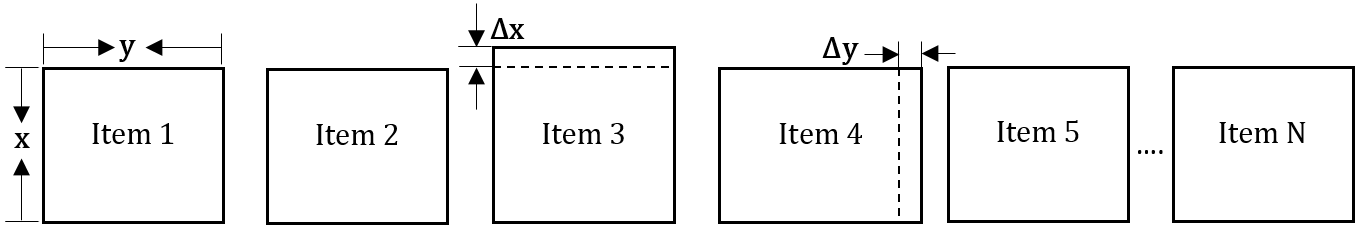
\includegraphics[width=0.9\textwidth]{size}
    \caption{Production batch in which item no.$3$ \& $4$ are oversized by $\Delta$x \& $\Delta$y units respectively.}
    \label{fig:size_line}
  \end{figure}

  \end{itemize}
\end{frame}

\subsection{Orientation}

% You can reveal the parts of a slide one at a time
% with the \pause command:
\begin{frame}{Orientation}{Eg: PCBs, Masks, Sub-parts etc.}
  \begin{itemize}
  \item Similarly, items produced by single process must be of same/specific orientation.
  \item Or no anomaly expected in the orientation.
  \begin{figure}
    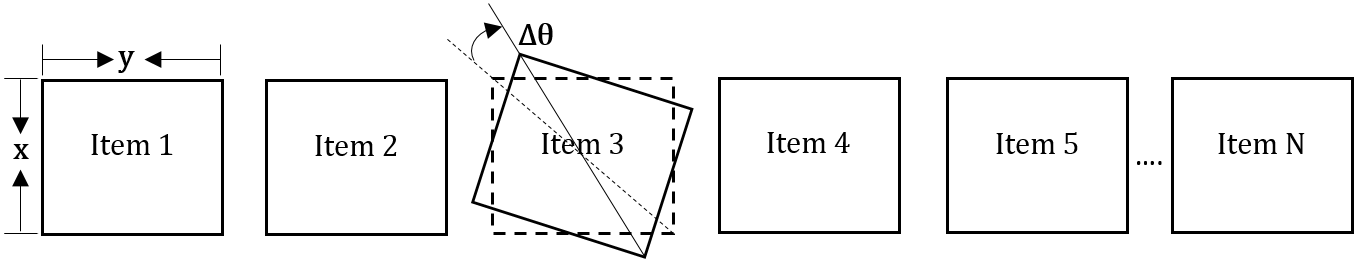
\includegraphics[width=0.9\textwidth]{orientation}
    \caption{Anomaly in the production of item no. $3$. The item has a defect in its orientation by an angle of $\Delta\theta^\circ$.}
    \label{fig:orientation_line}
  \end{figure}
  % You can also specify when the content should appear
  % by using <n->:
  %\item<3-> {
  %  Third item.
  %}
  %\item<4-> {
  %  Fourth item.
  %}
  % or you can use the \uncover command to reveal general
  % content (not just \items):
  %\item<5-> {
  %  Fifth item. \uncover<6->{Extra text in the fifth item.}
  %}
  \end{itemize}
\end{frame}

\subsection{Tolerance}

\begin{frame}{Tolerance}
  \begin{itemize}
  \item Needed for better judgement of quality of product.\\
  Eg: Allowance for $\Delta$x, $\Delta$y and $\Delta\theta$
  \item The errors occurred in measuring the parameters are due to actual physical error or analytical methods used or could be due to vibrations.
  \item It is important to know the source of error to precisely measure the parameters.
  \end{itemize}
\end{frame}

\subsection{Time}

\begin{frame}{Time}{Eg: Sorting in industries}
  \begin{itemize}
  \item Very crucial when the throughput is of importance.\\
  Eg: Japanese recycling industry. $2$ tonne in $1$ hr.!
  \item The decision making analytical methods must have low \\
  (or no) complexity.
  \item Linear models are preferable.
  \end{itemize}
\end{frame}


\section{Fault Detection using Multivariate Analysis}

\subsection{Production Model and Anomalies}

%\begin{frame}{Production Model}{Assumptions}
%  \begin{itemize}
%    \item Each product is scanned with a camera on top.
%    \item The image is thresholded using standard methods. \\
%    Eg: Otsu's global and Adaptive thresholds to mention a few.
%    \item A batch size of $N$ frames considered.
%    \item Images are sumulated with a series of binary images of size $50\times50$ pixels.
%  \end{itemize}
%  \begin{figure}
%    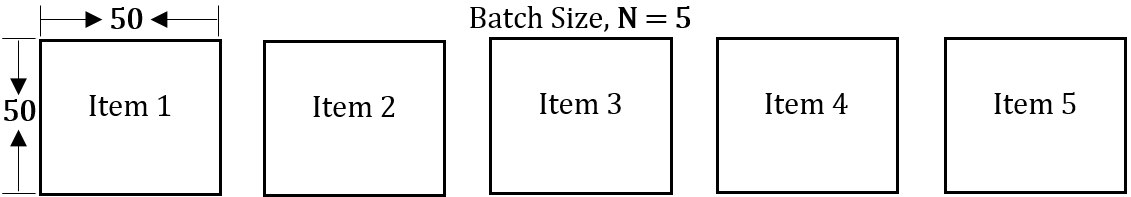
\includegraphics[width=0.8\textwidth]{model}
%  \end{figure}
%\end{frame}

\begin{frame}{Production Model and Anomalies}{Size and Orientation}
  \begin{figure}
    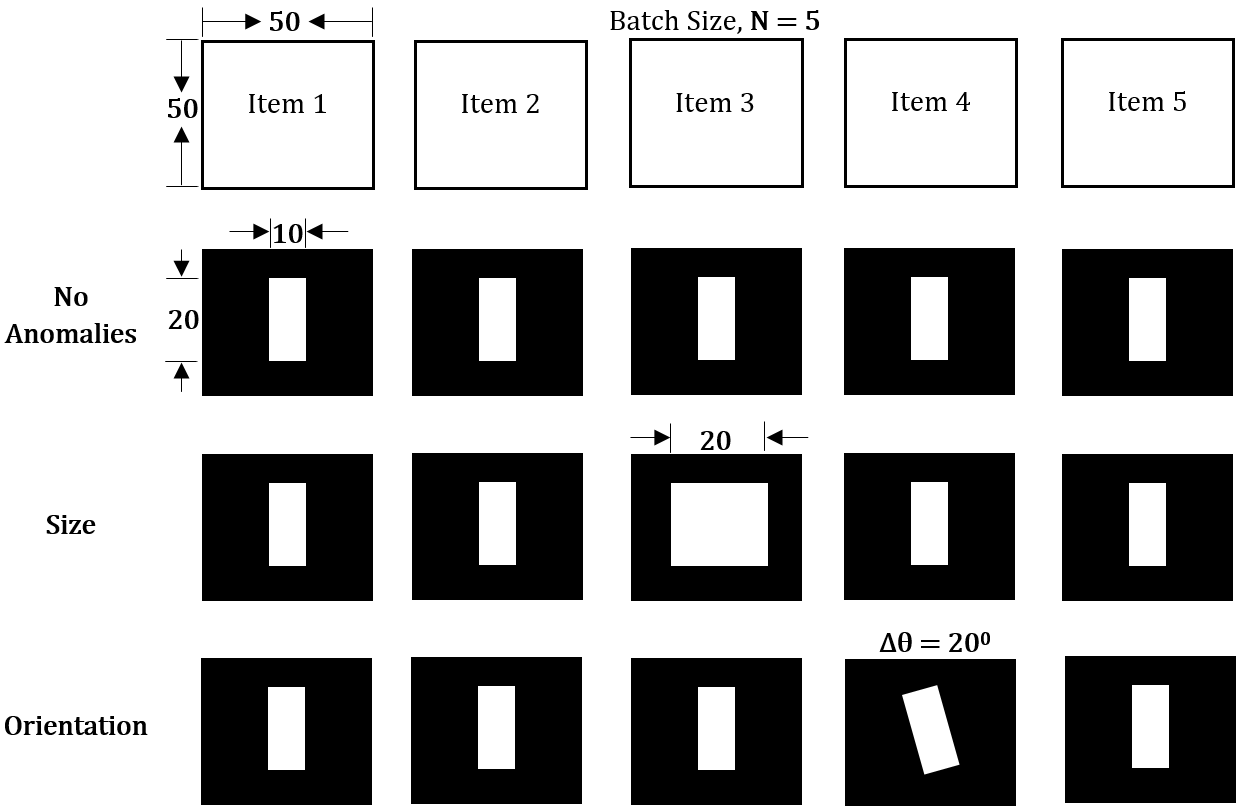
\includegraphics[width=0.8\textwidth]{anomalies_model}
  \end{figure}
\end{frame}

\subsection{Principle Component Analysis}

\begin{frame}{Anomaly due to change in Size}{Batch Size $N = 5$, with Gaussian noise, $\mathcal{N}(\mu,\sigma^2)=\mathcal{N}(0,0.25)$}
  \begin{figure}
    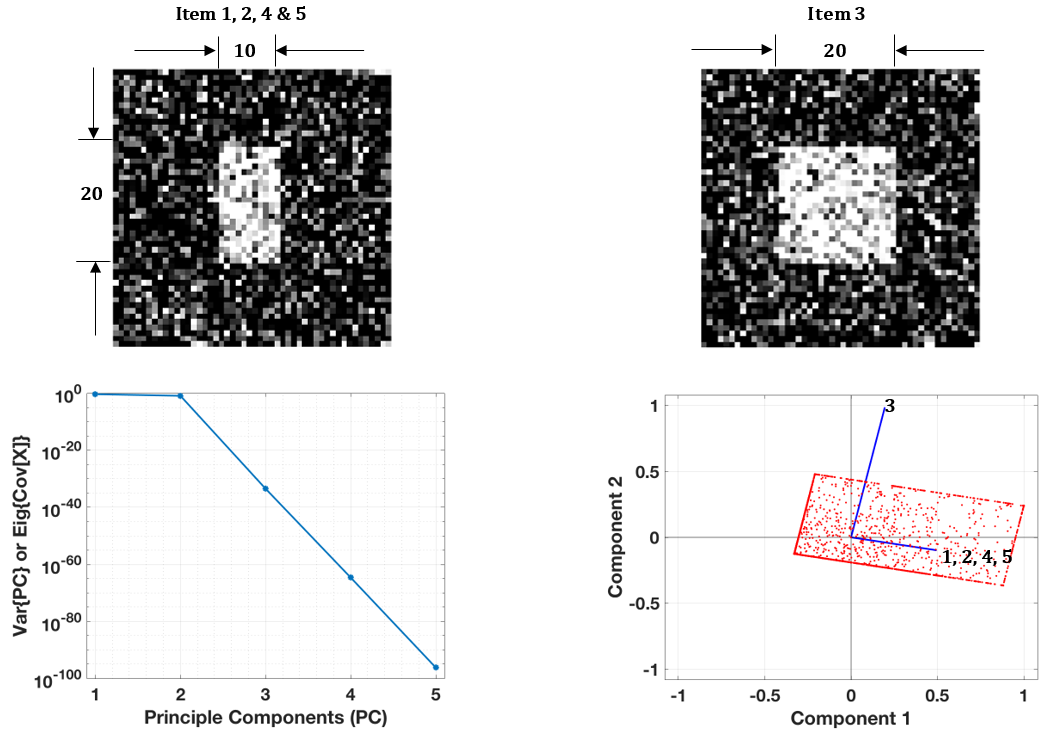
\includegraphics[width=1\textheight]{N5_Size_Detection}
  \end{figure}
\end{frame}

\begin{frame}{Anomaly due to change in Orientation}{Batch Size $N = 5$, with Gaussian noise, $\mathcal{N}(\mu,\sigma^2)=\mathcal{N}(0,0.25)$}
  \begin{figure}
    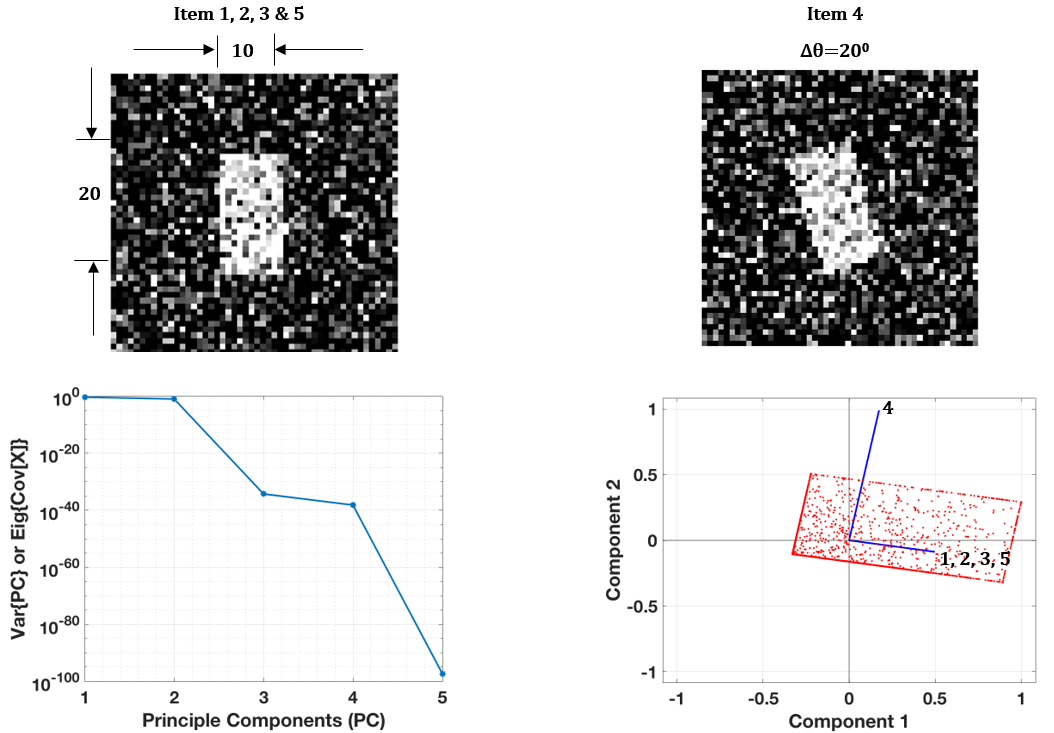
\includegraphics[width=1\textheight]{N5_Orientation_Detection}
  \end{figure}
\end{frame}

\subsection{Testing the robustness of the method}

\begin{frame}{Robustness of PCA}
  \begin{itemize}
    \item \texttt{nfaults}$ = $\texttt{randi}([1~5]); \texttt{\textcolor{gray}{\% Number of fault parts}} \\
    \texttt{\textcolor{gray}{\% -----------Random Size of Parts----------}}
    \item \texttt{sz1} = \texttt{randi}([1~\texttt{r}/2],~1,~\texttt{nfaults}); \texttt{\textcolor{gray}{\% Size rows}}
    \item \texttt{sz2} = \texttt{randi}([1~\texttt{c}/2],~1,~\texttt{nfaults}); \texttt{\textcolor{gray}{\% Size columns}}\\
    \texttt{\textcolor{gray}{\% -----------Random Orientation------------}}
    \item \texttt{rt} = \texttt{randi}([1~360],~1,~\texttt{nfaults}); \texttt{\textcolor{gray}{\% Rotation angles}} \\
    \texttt{\textcolor{gray}{\% -------Random location of faults---------}}
    \item \texttt{Pos} = \texttt{randi}([1~\texttt{N}],~1,~\texttt{nfaults}); \texttt{\textcolor{gray}{\% Locations in stack}}
  \end{itemize}
\end{frame}

\begin{frame}{Robustness of PCA: Size}{Batch Size $N = 100$, with Gaussian noise, $\mathcal{N}(\mu,\sigma^2)=\mathcal{N}(0,2)$}
  \begin{figure}
    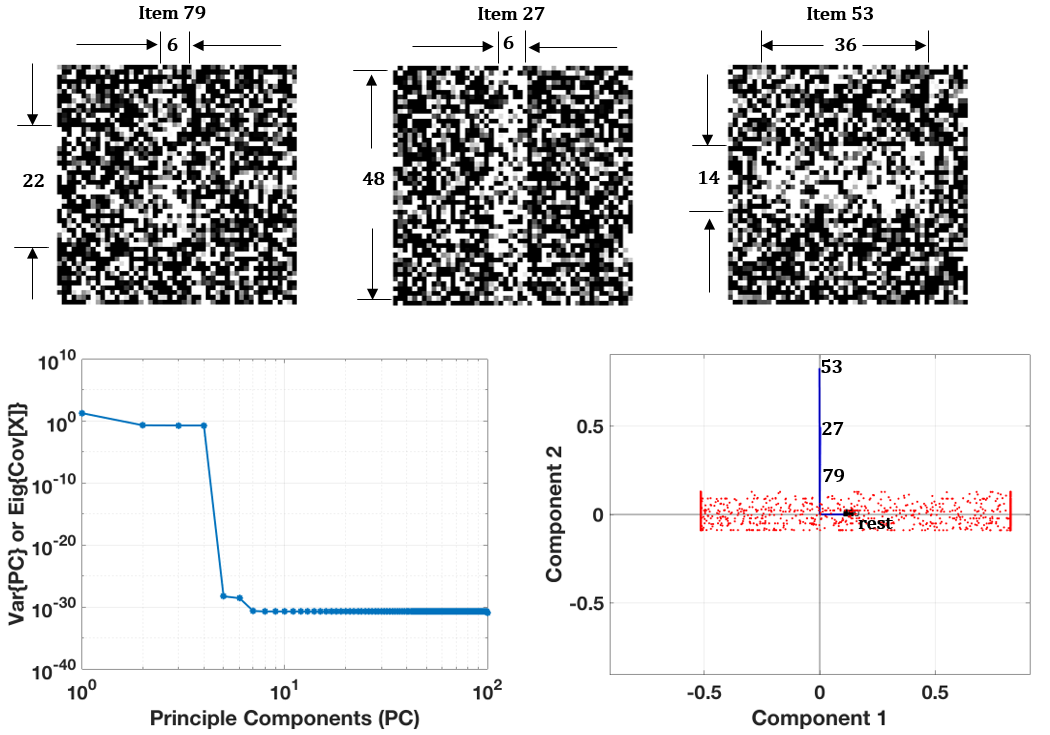
\includegraphics[width=1\textheight]{Random_Size_Detection}
  \end{figure}
\end{frame}

\begin{frame}{Robustness of PCA: Orientation}{Batch Size $N = 100$, with Gaussian noise, $\mathcal{N}(\mu,\sigma^2)=\mathcal{N}(0,2)$}
  \begin{figure}
    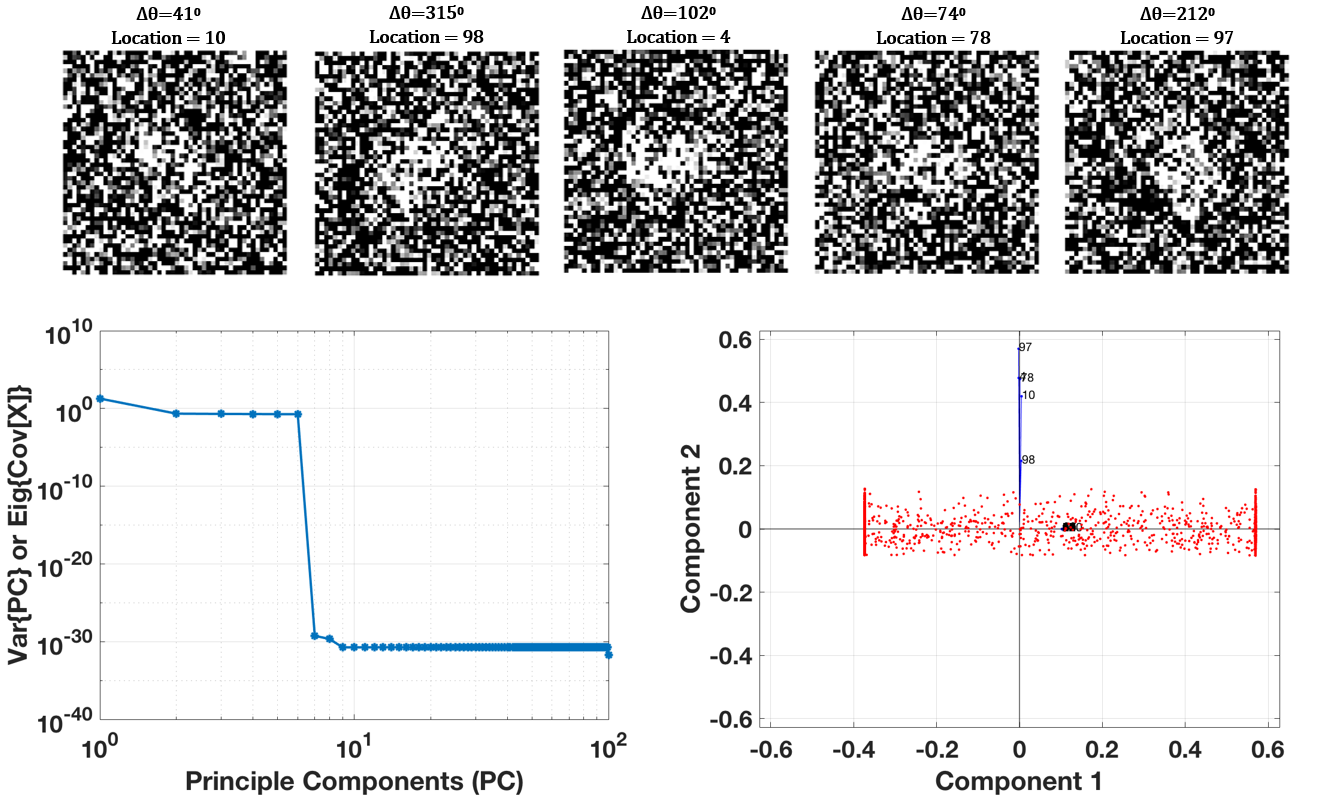
\includegraphics[width=1\textheight]{Random_Orientation_Detection}
  \end{figure}
\end{frame}

%\begin{frame}{Blocks}
%\begin{block}{Block Title}
%You can also highlight sections of your presentation in a block, with it's own title
%\end{block}
%\begin{theorem}
%There are separate environments for theorems, examples, definitions and proofs.
%\end{theorem}
%\begin{example}
%Here is an example of an example block.
%\end{example}
%\end{frame}

% Placing a * after \section means it will not show in the
% outline or table of contents.
\section*{Summary}

\begin{frame}{Summary}
  \begin{itemize}
  \item The PCA method is robust in identifying abnormalities in the process.
  \item \alert{Random} number of faulty images and their locations, $\Delta\theta$ and Sizes have been tested.
  \item PCA is a linear model. \alert{Fast} decision maker.
  \item \alert{Simpler}, \alert{Cost effective} metrological method of fault detection in manufacturing and quality control.
  \end{itemize}

  \begin{itemize}
  \item
    Outlook
    \begin{itemize}
    \item The extent of abnormalities can be studied in depth in Endmember extraction methods such as Vertex Component Analysis (VCA) and random N-findr extraction.
    \end{itemize}
  \end{itemize}
\end{frame}



% All of the following is optional and typically not needed.
\appendix
\section<presentation>*{\appendixname}
\subsection<presentation>*{For Further Reading}

\begin{frame}[allowframebreaks]
  \frametitle<presentation>{Open Source Data}

  \begin{thebibliography}{10}

  \beamertemplatebookbibitems
  % Start with overview books.

  \bibitem{vcangadi1}
    GitHub: vcangadi1
    \newblock {\em Matlab~Codes, Documentation, \LaTeX~Slides and Data}.
    \newblock https://github.com/vcangadi1/Presentations


  %\beamertemplatearticlebibitems
  % Followed by interesting articles. Keep the list short.

  %\bibitem{Someone2000}
  %  S.~Someone.
  %  \newblock On this and that.
  %  \newblock {\em Journal of This and That}, 2(1):50--100,
  %  2000.
  \end{thebibliography}
\end{frame}

\end{document}
